%%%%%%%%%%%%%%%%%%%%%%%%%%%%%%%%%%%%%%%%%
% Journal Article
% LaTeX Template
% Version 1.4 (15/5/16)
%
% This template has been downloaded from:
% http://www.LaTeXTemplates.com
%
% Original author:
% Frits Wenneker (http://www.howtotex.com) with extensive modifications by
% Vel (vel@LaTeXTemplates.com)
%
% License:
% CC BY-NC-SA 3.0 (http://creativecommons.org/licenses/by-nc-sa/3.0/)
%
%%%%%%%%%%%%%%%%%%%%%%%%%%%%%%%%%%%%%%%%%

%----------------------------------------------------------------------------------------
%	PACKAGES AND OTHER DOCUMENT CONFIGURATIONS
%----------------------------------------------------------------------------------------

\documentclass[twoside,twocolumn]{article}
\usepackage[UTF8]{ctex}
\usepackage{graphicx}
\usepackage{blindtext} % Package to generate dummy text throughout this template

\usepackage[sc]{mathpazo} % Use the Palatino font
\usepackage[T1]{fontenc} % Use 8-bit encoding that has 256 glyphs
\linespread{1.05} % Line spacing - Palatino needs more space between lines
\usepackage{microtype} % Slightly tweak font spacing for aesthetics

\usepackage[english]{babel} % Language hyphenation and typographical rules

\usepackage[hmarginratio=1:1,top=32mm,columnsep=20pt]{geometry} % Document margins
\usepackage[hang, small,labelfont=bf,up,textfont=it,up]{caption} % Custom captions under/above floats in tables or figures
\usepackage{booktabs} % Horizontal rules in tables

\usepackage{lettrine} % The lettrine is the first enlarged letter at the beginning of the text

\usepackage{enumitem} % Customized lists
\setlist[itemize]{noitemsep} % Make itemize lists more compact

\usepackage{abstract} % Allows abstract customization
\renewcommand{\abstractnamefont}{\normalfont\bfseries} % Set the "Abstract" text to bold
\renewcommand{\abstracttextfont}{\normalfont\small\itshape} % Set the abstract itself to small italic text

\usepackage{titlesec} % Allows customization of titles
\renewcommand\thesection{\Roman{section}} % Roman numerals for the sections
\renewcommand\thesubsection{\roman{subsection}} % roman numerals for subsections
\titleformat{\section}[block]{\large\scshape\centering}{\thesection.}{1em}{} % Change the look of the section titles
\titleformat{\subsection}[block]{\large}{\thesubsection.}{1em}{} % Change the look of the section titles

\usepackage{fancyhdr} % Headers and footers
\pagestyle{fancy} % All pages have headers and footers
\fancyhead{} % Blank out the default header
\fancyfoot{} % Blank out the default footer
\fancyhead[C]{Running title $\bullet$ May 2016 $\bullet$ Vol. XXI, No. 1} % Custom header text
\fancyfoot[RO,LE]{\thepage} % Custom footer text

\usepackage{titling} % Customizing the title section

\usepackage{hyperref} % For hyperlinks in the PDF

%----------------------------------------------------------------------------------------
%	TITLE SECTION
%----------------------------------------------------------------------------------------

\setlength{\droptitle}{-4\baselineskip} % Move the title up

\pretitle{\begin{center}\Huge\bfseries} % Article title formatting
\posttitle{\end{center}} % Article title closing formatting
\title{稀土的应用与发展趋势} % Article title
\author{%
\textsc{杨建熙}\thanks{A thank you or further information} \\[1ex] % Your name
\normalsize 桂林理工大学 \\ % Your institution
\normalsize \href{mailto:john@smith.com}{john@smith.com} % Your email address
%\and % Uncomment if 2 authors are required, duplicate these 4 lines if more
%\textsc{Jane Smith}\thanks{Corresponding author} \\[1ex] % Second author's name
%\normalsize University of Utah \\ % Second author's institution
%\normalsize \href{mailto:jane@smith.com}{jane@smith.com} % Second author's email address
}
\date{\today} % Leave empty to omit a date
\renewcommand{\maketitlehookd}{%
\begin{abstract}
\noindent
\blindtext

\end{abstract}
}

%----------------------------------------------------------------------------------------

\begin{document}

% Print the title
\maketitle

%----------------------------------------------------------------------------------------
%	ARTICLE CONTENTS
%----------------------------------------------------------------------------------------

\section{稀土简介}
稀土(Rare Earth),是化学周期表中镧系元素和钪、钇共十七种金属元素的总称。有着“工业维生素”的美称。稀土的应用范围广泛,在军事、工业、农业、医学方面都有着相当重要的用途,尤其是随着现代电子信息技术的发展,稀土的用途也逐渐向高新科技领域迈进,成为了必不可少的原材料。中国已经成为了世界上中国已经成为世界上唯一的可以大量供应不同品种及不同品级稀土产品的国家, 在世界稀土市场上具有支配和主导地位,并且有着完善的产业链,同时稀土作为我国的战略资源,因此我们有必要研究稀土的经济价值与前景。
\section{我国稀土的分布和现状}

\lettrine[nindent=0em,lines=3]{我}{国}
是世界稀土资源大国, 据1993 年1月美国矿物局出版的统计资料表明, 世界稀土工业储量为1 亿吨( REO ), 中国为430 万吨, 占世界总储量的43$\%$。我国稀土资源的特点是储量大、类型多、品种全、质量好、开采成本低,目前开发利用的稀土矿物主要有五种:氟碳铈矿、离子吸附型稀土矿、独居石矿、磷钇矿和磷灰石矿, 前四种矿占世界稀土产量的95 $\%$以上。除Pm 外的16 个稀土元素, 在我国从南到北分布齐全。中国稀土矿主要有白云鄂博矿, 四川冕宁矿, 山东微山矿, 南方七省的离子吸附型稀土矿, 广东、广西、江西的磷钇矿, 湖南、广东、广西、海南、台湾的独居石矿, 贵州含稀土的磷矿, 长江重庆段淤砂中的钪矿, 以及漫长海岸线上的海滨砂矿等。目前已形成了良好的生产布局, 产量稳居世界首位。

虽然我国的稀土资源居世界第一,但由于稀土应用水平较低等原因,我国稀土资源产业长期存在资源过度开采、大范围低价输出、不当开采引发环境污染难以处理等问题,资源优势没有相应产业化为经济优势。近些年来,稀土在整个国家发展中发挥了日益显著的作用,稀土问题越来越受到政府的高度重视,相继出台了一系列政策措施,在提高稀土出口价格、防治过度开采等方面取得了一定的进展。但稀土开采带来生态环境破坏以及滥采乱挖等问题仍然未能根治。
\begin{figure}[h]
  \centering
  \includegraphics[width=20em]{figure2.png}
  \caption{中国稀土矿床(点)分布图}
\end{figure}

%------------------------------------------------

\section{稀土的应用领域}

\subsection{冶金领域}
稀土在钢铁冶金中的应用是中国稀土的最大消费领域,特别是在铸铁中的应用很普遍,从1991年到1995年呈逐年增长的的趋势,在钢中的应用相应的小一些,而且需求逐年减少。稀土在铸铁中的作用主要是作为球化剂、蠕化剂和孕育剂使用; 在钢中的作用主要是脱硫、脱氧、细化晶粒、去除杂质等作用,从而改善钢的各项力学性能。由于稀土金属有着很高的化学活性和较大的原子半径,将其应用在有色金属及合金中能起到改善合金的作用。我国在有色金属中应用稀土起步较晚,但是该领域的需求逐年增长尤其是稀土铝合金和稀土镁合金,一直受到国家是重视。
\subsection{石油化工领域}
目前,这一领域消费稀土最多的是石油催化裂化,年消费稀土1万余吨,还有数百吨稀土用于各种涂料与颜料等领域。1962年,美孚石油公司研究发现,稀土可加速石油大分子的裂化进程,稀土不仅可增加催化剂的活性,保持催化剂的热稳定性,还可增加设备的原油处理量,提高汽油产出率,降低炼油成本。此后,稀土在石油催化裂化剂中的应用迅速展开,到1983年,美国消费于这一领域的稀土量增加到12700吨REO,占稀土总消费量( 19600吨REO )的65$\%$ 。
\subsection{玻璃领域}
这是稀土应用量大,花色品种繁多的领域。稀土用于玻璃有百多年的历史, 19世纪末, 稀土开始用于玻璃作脱色澄清剂、着色剂,后来用于镜头玻璃、玻璃抛光(稀土抛光粉在本文“新材料”部分中叙述)。后来发展到用于光导纤维、防紫外线。防幅射、硬盘玻璃基片以及其它特种玻璃。现在看来,消费稀土量最多的是脱色澄清剂与镜头玻璃(不包括抛光粉)。据称2000年全球用于CRT(阴极射线管)玻璃中的稀土达1万吨。
\subsection{发光材料}
由于稀土离子具有丰富的能级和4f电子跃迁特性使稀土成为一个巨大的发光宝库,为高新技术领域提供了很多性能优越的发光材料和激光材料。
\subsection{永磁材料}
稀土永磁材料的发展大致经历了三个时代,即:60年代发明的第一代水磁体SmCo3;由于Co的价格昂贵,即而开发出来了Sm2Co1型第二代永磁体,最大磁能积可达240kJ/m3(40GOe),性能稳定,温度稳定性和耐腐蚀性都很好,是一种主要的水磁体;1983年美国和日本相继发明了物美价廉的Nd Fe一B第三代永磁体,其理论磁能积为512kJm3(64MGOe),实际目前已达到432kJ/m3(5MGOe),是目前世界上磁性最强的永磁体。现在人们又在致力研究开发Sm-Fe-N系等永磁材料,有望成为第四代稀土永磁材料。目前飞速发展的电子计算机、磁电式仪表、磁悬浮系统等都已成为稀土永磁体的主要应用领域。初步统计,我国目前稀土永磁材料生产企业有200多家,总生产能力约2000吨/年。预计随着科技的发展,稀土永磁材料的用量将不断增加。
\subsection{医学领域}
稀土化合物在抗凝血方面占有特别地位,这些化合物在体内外都能降低血液的凝固,特别是静脉注射,其抗凝血作用立即产生并且能持续一天左右。低浓度的稀土化合物水溶液具有抑菌和抗炎作用,可以用作烧伤药物。给活体注入稀土盐的一个明显的生理作用是引起低血糖,因而促使人们对稀土用于治疗糖尿病的研究。同时稀土元素还具有抗癌作用,用稀土放射性同位素。1965年 Haley阐明用稀土放射性同位素可以治疗与垂体有关的肿瘤,由于垂体在肿瘤的生成中起重要作用,人们常有选择地将稀土放射性同位素作用于垂体以控制某些疾病。
Text requiring further explanation\footnote{Example footnote}.

\section{稀土的发展趋势分析}
中国对稀土的运用始于20 世纪60 年代中期在铸铁中的应用, 不久, 在钢中也得到应用,但是早期由于技术水平发展的落后,稀土主要作为原材料卖给国外,仅仅能获得微薄的利润。随着新兴产业的发展,稀土广泛应用于电子、能源、交通、航天、农业、医疗等13个经济领域的40多个行业,尤其对中重稀土的需求不断增加。
\begin{figure}[h]
  \centering
  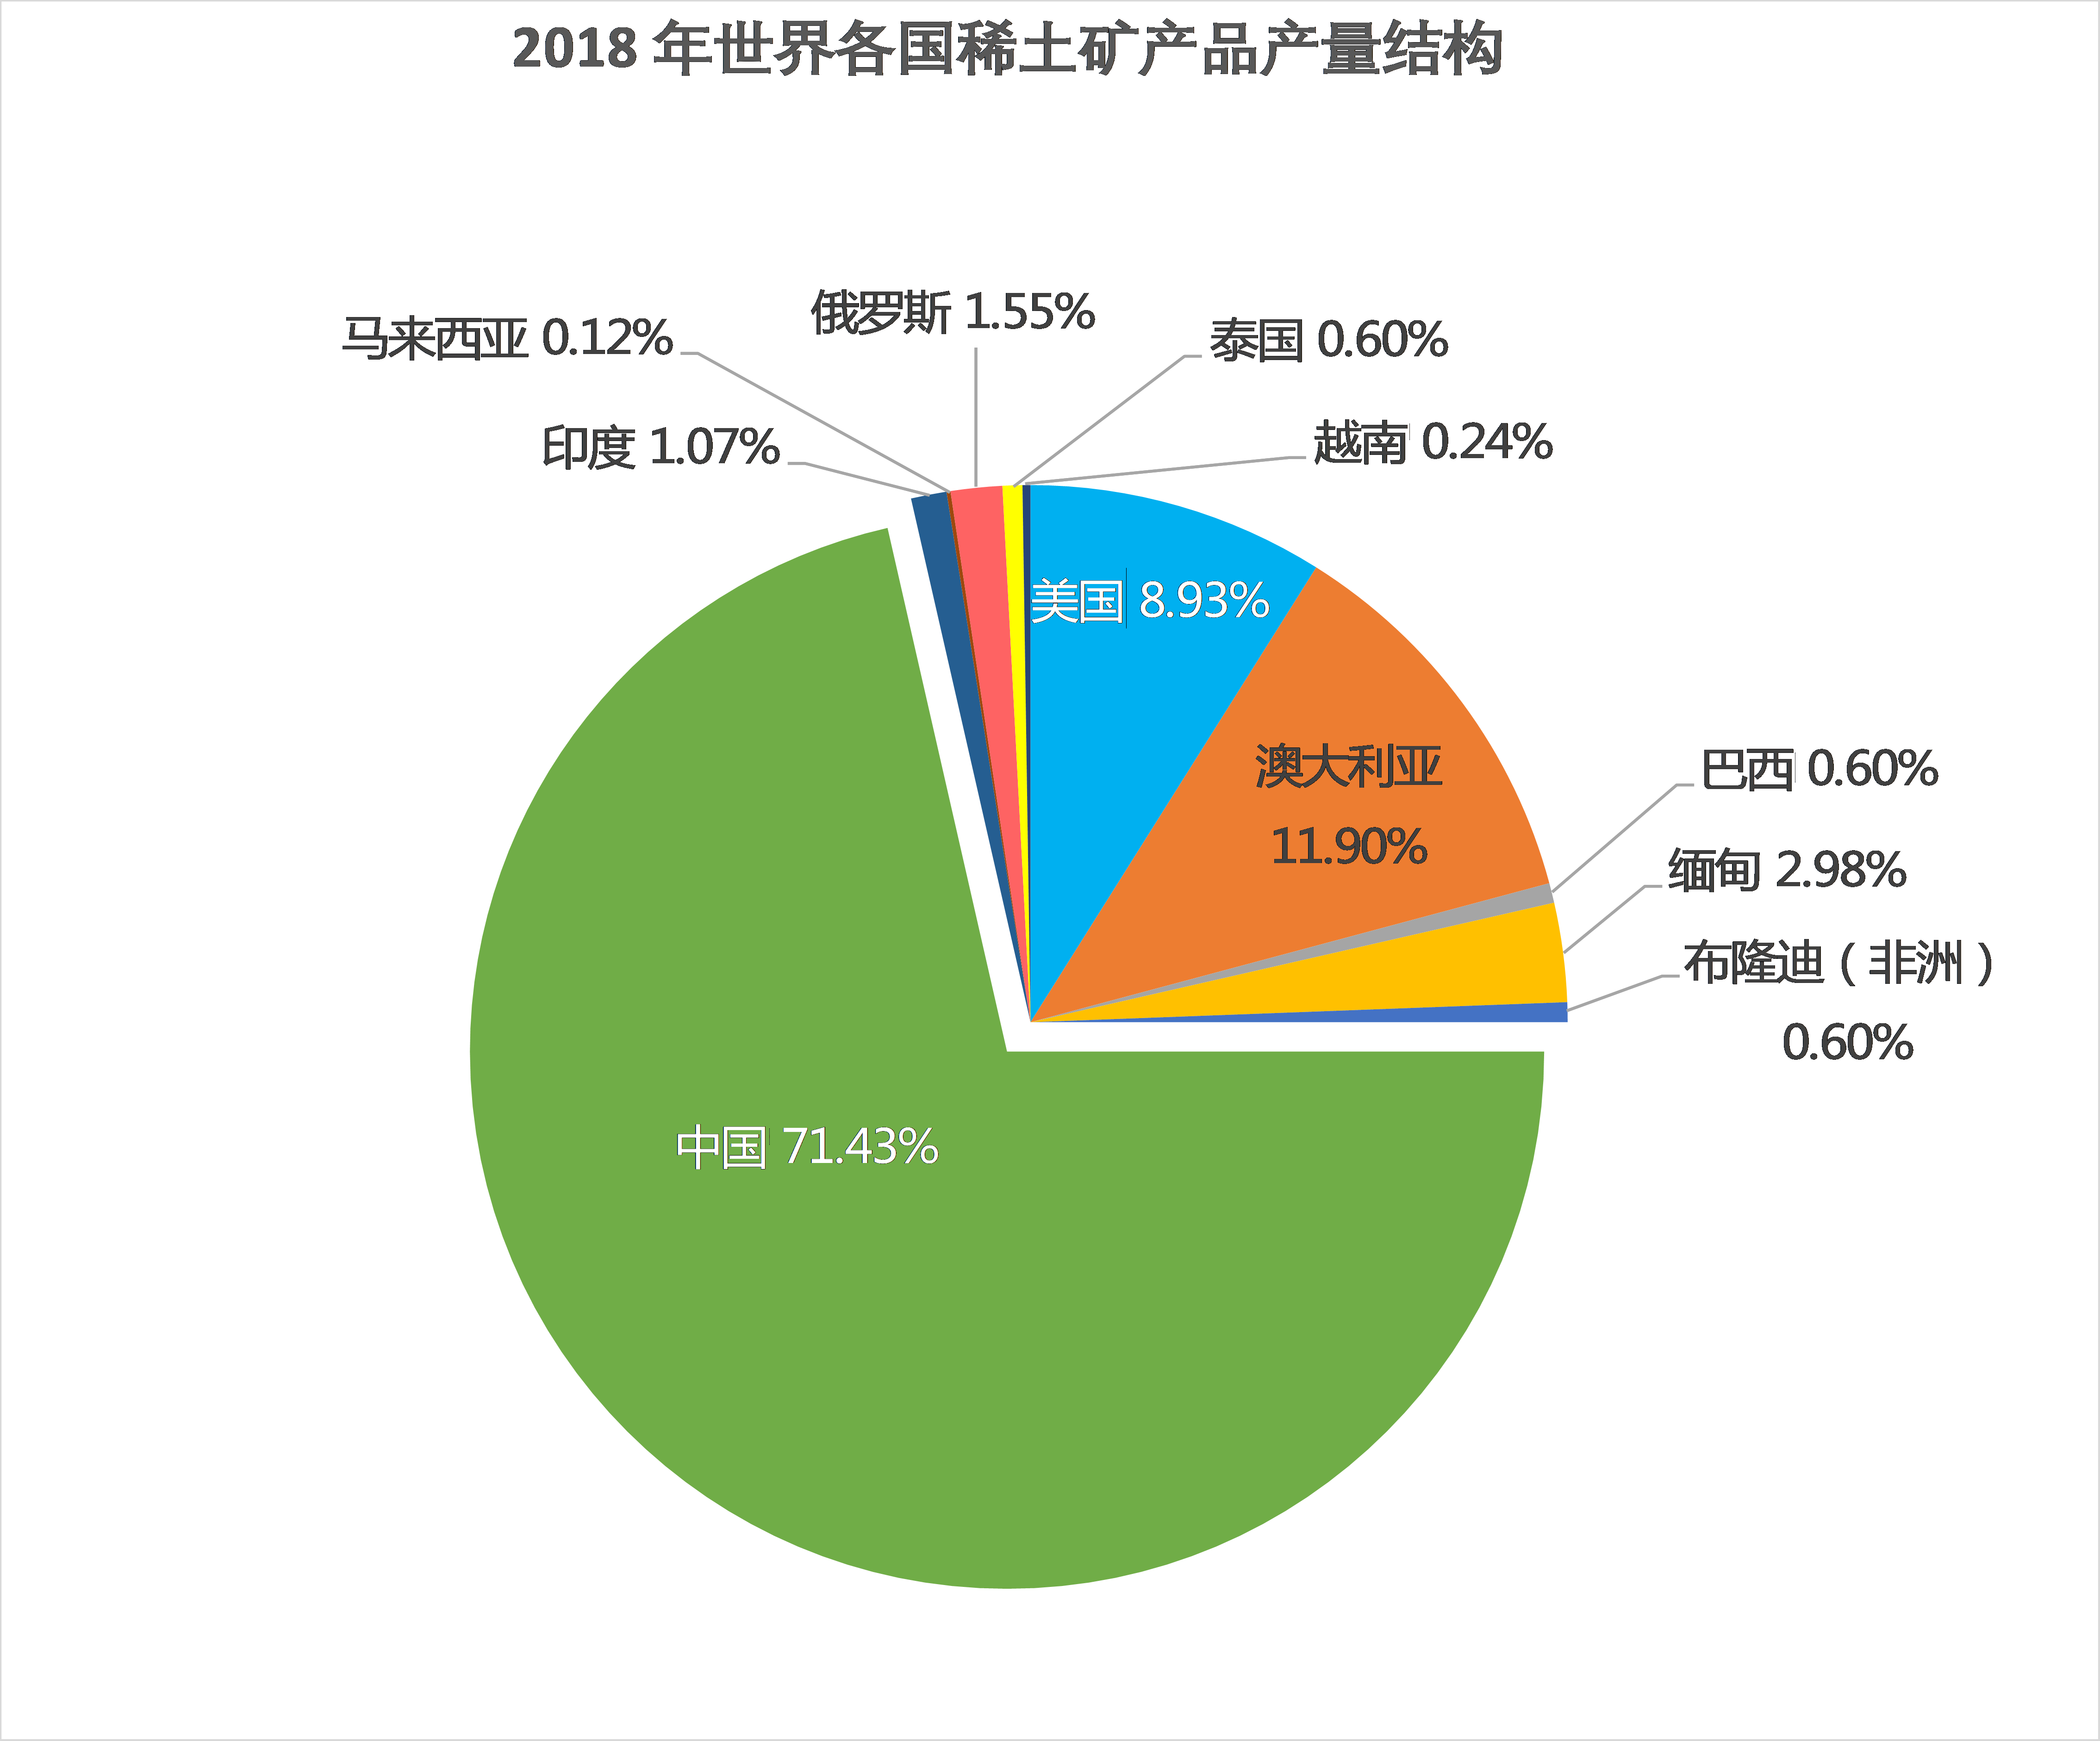
\includegraphics[width=20em]{figure1.png}
  \caption{2018 年世界各国稀土矿产品产量结构}
\end{figure}
综上所述,从近年来世界范围内稀土的供应来源看,供应国家逐渐增加; 除中国外其他国家的供应总量将逐渐增加; 中国稀土供应比例将下降,世界稀土矿产品的供应将呈现多元化的供应格局与趋势。
通过上述分析可见, 稀土产业与高新技术产业关联度密切, 产品市场全球化特点突出, 其后续产业链的发展空间也十分广阔, 是21 世纪的朝阳产业。


%------------------------------------------------

\section{结论}

\begin{table}
\caption{Example table}
\centering
\begin{tabular}{llr}
\toprule
\multicolumn{2}{c}{Name} \\
\cmidrule(r){1-2}
First name & Last Name & Grade \\
\midrule
John & Doe & $7.5$ \\
Richard & Miles & $2$ \\
\bottomrule
\end{tabular}
\end{table}

\blindtext % Dummy text

\begin{equation}
\label{eq:emc}
e = mc^2
\end{equation}

\blindtext % Dummy text

%------------------------------------------------

\section{Discussion}

\subsection{Subsection One}

A statement requiring citation \cite{Figueredo:2009dg}.
\blindtext % Dummy text

\subsection{Subsection Two}

\blindtext % Dummy text

%----------------------------------------------------------------------------------------
%	REFERENCE LIST
%----------------------------------------------------------------------------------------

\begin{thebibliography}{99} % Bibliography - this is intentionally simple in this template

\bibitem[Figueredo and Wolf, 2009]{Figueredo:2009dg}
Figueredo, A.~J. and Wolf, P. S.~A. (2009).
\newblock Assortative pairing and life history strategy - a cross-cultural
  study.
\newblock {\em Human Nature}, 20:317--330.

\end{thebibliography}

%----------------------------------------------------------------------------------------

\end{document}
